\subsubsection{Identified particle \vn}\label{sec:identified_particle_vn}


\begin{figure}[!htb]
\begin{center}
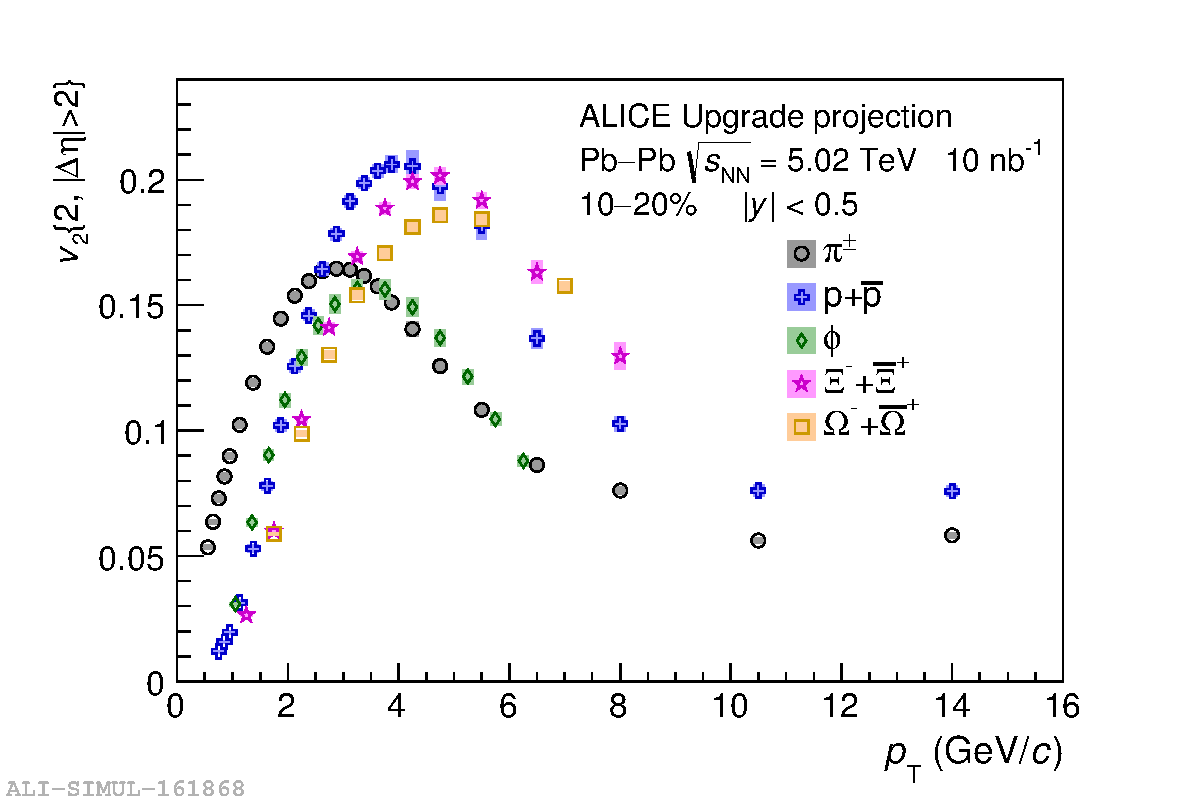
\includegraphics[width=0.495\textwidth]{\main/flow/figs/alice_projection_pid_v2}
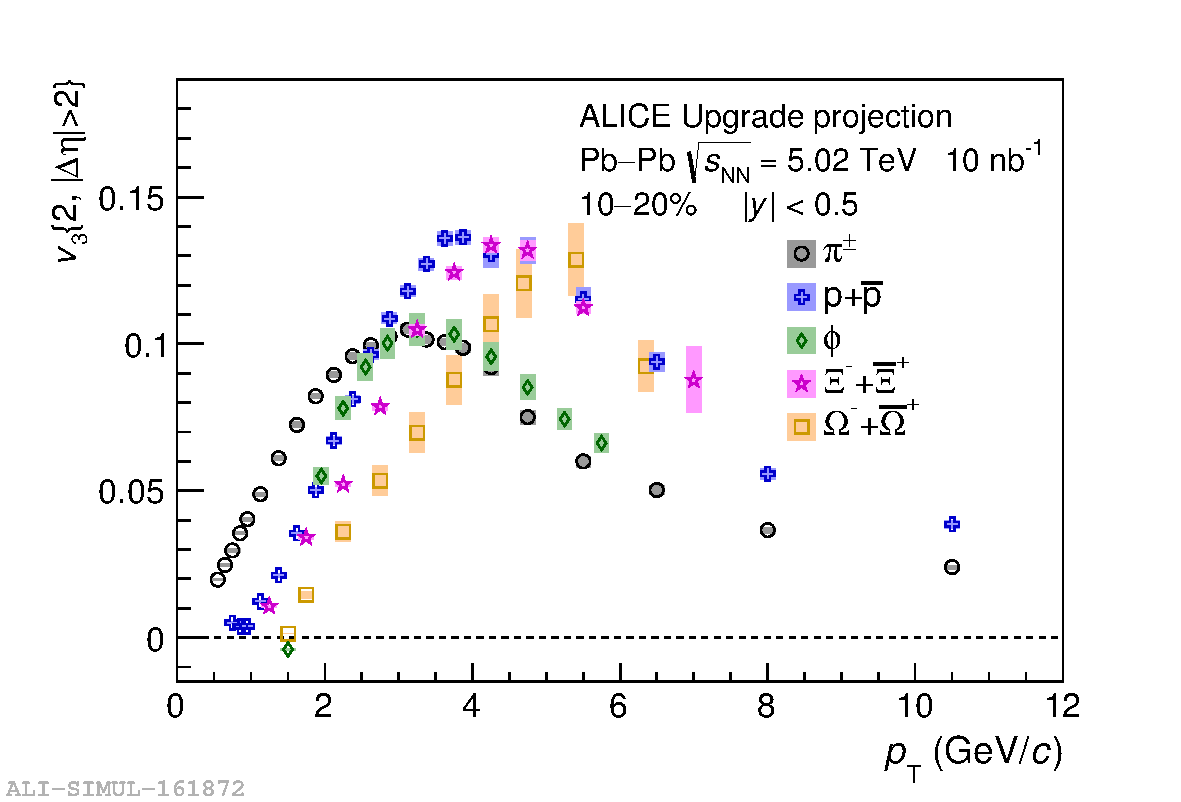
\includegraphics[width=0.495\textwidth]{\main/flow/figs/alice_projection_pid_v3}
\caption{
ALICE projections for $v_2$ (left) and $v_3$ (right) of $\pi^\pm$, 
  $\mathrm{p}$+$\overline{\mathrm{p}}$, $\Xi$+$\overline{\Xi}$, 
  $\Omega$+$\overline{\Omega}$, and the $\phi$-meson 
  in the 10--20\% centrality interval
  for an integrated luminosity of 10~nb$^{-1}$. 
Error bars (shaded boxes) represent the projected statistical 
  (systematic) uncertainties.}
\label{fig:alice_vn}
\end{center}
\end{figure}

As stated earlier most \vn\ measurements for inclusive hadrons are the LHC 
  are not statistics limited.
However for identified particles there is considerable scope for reduction 
  in statistical uncertainties in Run~3 and 4.
This is true both for heavy-flavor particles 
  as well for identified light flavour hadrons.
Figure~\ref{fig:alice_vn} shows projections from the ALICE collaboration for 
  the $v_2$ and $v_3$ of several light-flavor species, that are expected for 
  an integrated luminosity of 10~nb$^{-1}$ expected in Run~3 and 4.
The projected statistical uncertainties are typically negligible over the 
  entire \pt\ range and in most cases the systematic uncertainties are 
  quite small as well.

As stated before, the increased precision of these measurements will help in 
  better understanding of the QGP equation of state. 
These measurements will also lead to an improved understanding 
  of the hadronization mechanism at the QGP$\rightarrow$hadron transition.
Additionally, detailed measurements of constituent quark scaling (or its violation)
  can provide constraints on the contribution of the subsequent hadronic 
  rescattering, to the final azimuthal anisotropy of the final particles.
This is because the azimuthal anisotropy developed in the QGP phase 
  is expected to scale with the 
  number of constituent quarks, while the anisotropy developed in the hadronic
  phase is different for different particle species, depending on the particle 
  mass and hadronic coss-section.


\begin{figure}[!htb]
\begin{center}
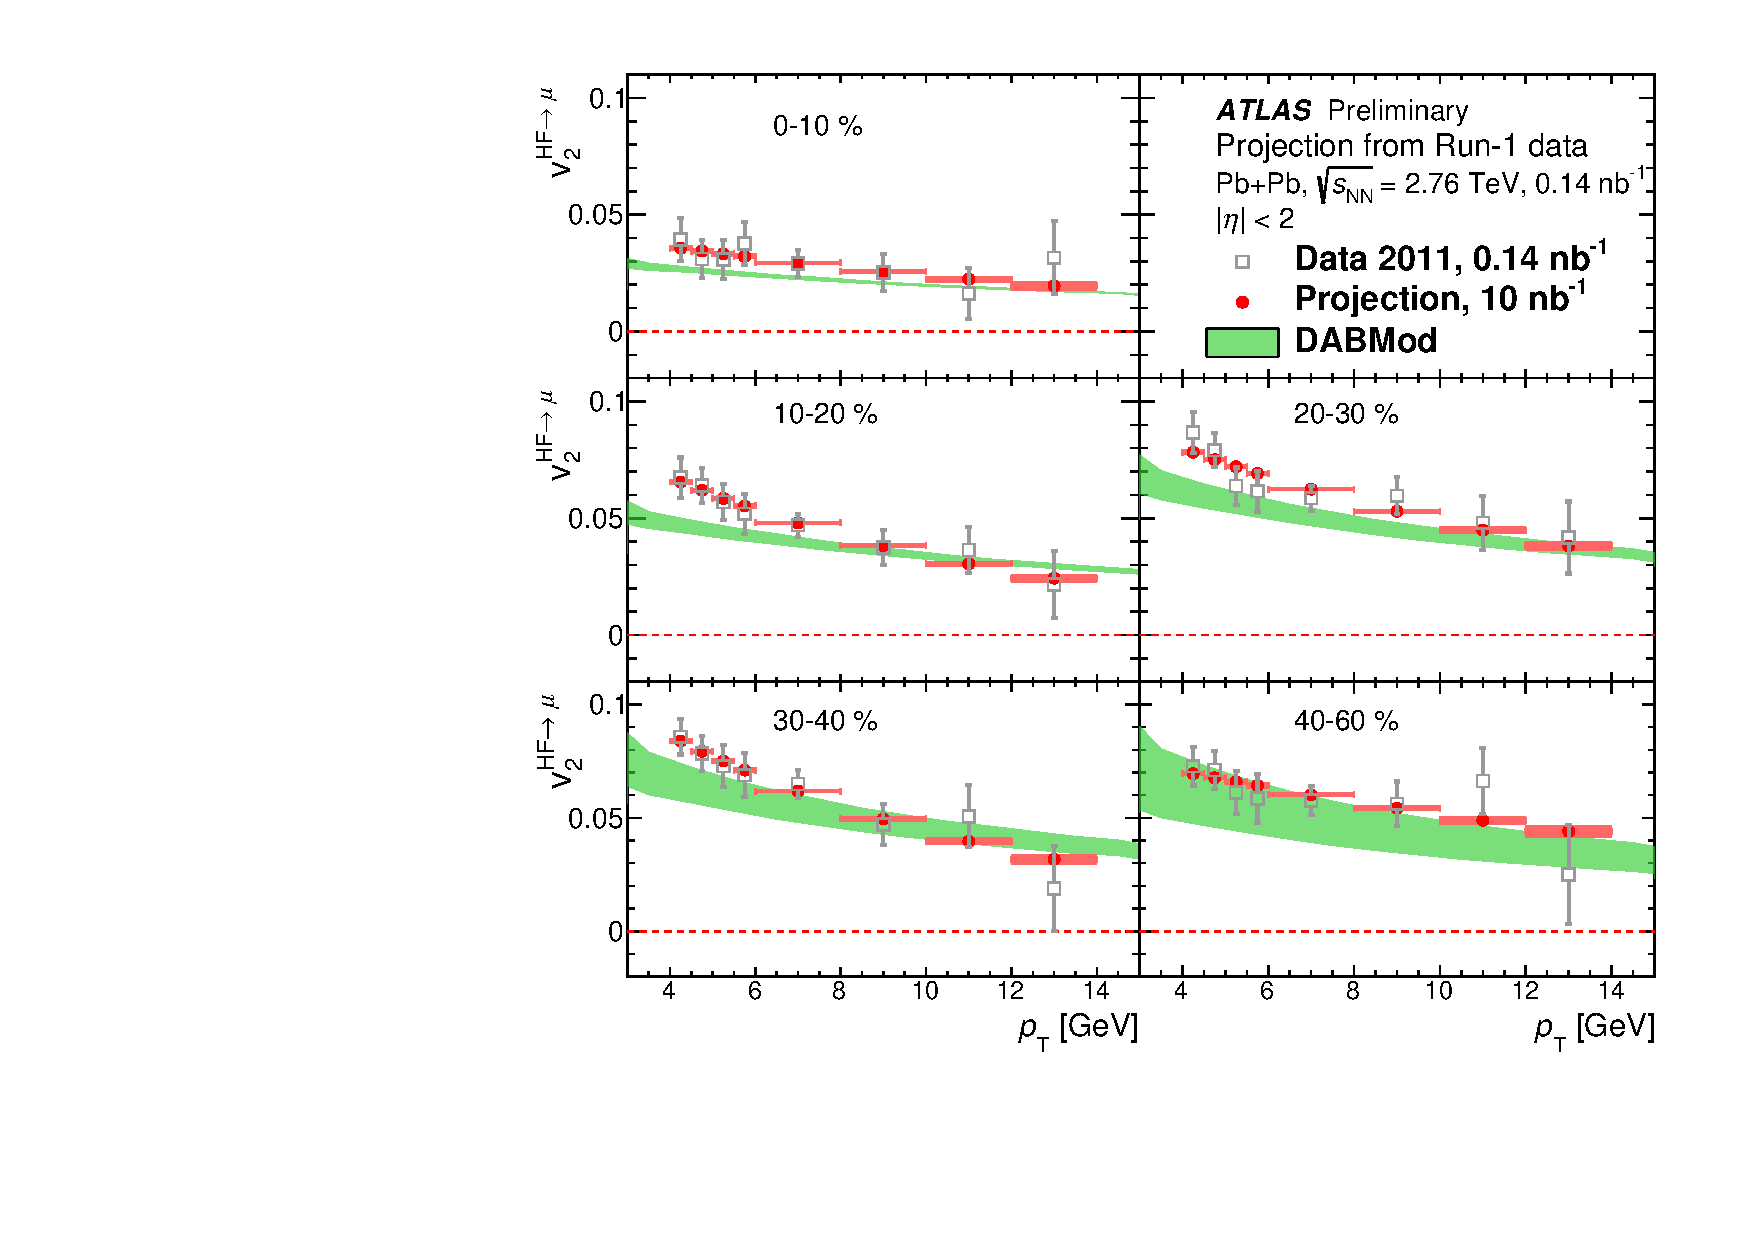
\includegraphics[width=1.0\textwidth]{\main/flow/figs/atlas_hfmuonv2}
\caption{
ATLAS projections of $v_2$ as a function of \pt, for muons from the decay of 
  heavy-flavor hadrons. 
Each panel corresponds to a different centrality interval. 
The present measurements are also shown for comparison. 
The error bars (shaded boxes) correspond to statistical uncertainties only. 
The projections are also compared to calculations from the DABMod model.}
\label{fig:atlas_hf_v2}
\end{center}
\end{figure}

Figure~\ref{fig:atlas_hf_v2} shows projections from the ATLAS collaboration
  for the $v_2$ of muons produced from the decay of heavy-flavor hadrons
  in Run~3 and 4, showing a considerable improvement in the statitical 
  precision of the measurement.
The central values of the projections are obtained by fitting the 
  present measurements with an exponential function, which qualitatively 
  describes the present data. 
The statistical uncertainties in the projections are made by scaling down 
  the present uncertainties to correspond to the expected luminosity in 
  Run~3 and 4 (10~nb$^{-1}$).
Calculations from the DABMod model~\cite{Prado:2016szr} are also shown,
  which demonstrate the inability of the present measurements
  in establishing or ruling out models due to limited statistical precision.
The flow measurements for heavy quarks is important as they are produced at
  earlier times in the heavy-ion collision and thus are susceptible
  to the full time evolution of the QGP.
The heavy-flavor anisotropy measurements can determine if heavy-quarks couple 
  strongly or weakly to the QGP, and additionally can constrain the heavy-quark 
  transport and diffusion coefficients.
Chapter~\ref{sec:HI_HF} has further discussions of Run~3 and 4 flow projections
  for heavy-flavor particles and their physics implications. 


